% Relatório da Avaliação A2 (versão revisada) — template IEEEtran (conference)
% Compilar no Overleaf com pdfLaTeX. As figuras devem estar em "figuras/" ou em "Modelagem_A2/figuras/".
\documentclass[conference]{IEEEtran}
\IEEEoverridecommandlockouts
\usepackage[utf8]{inputenc}
\usepackage[T1]{fontenc}
\usepackage[brazil]{babel}
\usepackage{graphicx,amsmath,booktabs,url,array}
\graphicspath{{figuras/}{Modelagem_A2/figuras/}}
\renewcommand{\IEEEkeywordsname}{Palavras-chave}
\begin{document}
\title{Vazamento de informação na triagem de laudos cardiológicos pediátricos: o que sobra quando o exame físico sai}
\author{\IEEEauthorblockN{Jamily Vieira, Júlia Souza, Yasmin Mageste}
\IEEEauthorblockA{Instituto de Informática, Universidade Federal de Goiás\\Mineração de Dados -- Avaliação A2}
\thanks{Código e dados para reprodução: \protect\url{https://github.com/Julia-PS24/mineracao_de_dados} (random\_state = 42 em todas as etapas).}}
\maketitle

\begin{abstract}
Este trabalho investiga se o laudo de uma consulta de cardiologia pediátrica pode ser previsto apenas com o que se sabe antes do exame do especialista, usando 10.576 consultas do Real Hospital Português, em Recife. A análise exploratória revelou vazamento de informação: sopro, segunda bulha e pulsos são anotados no mesmo exame que gera o rótulo, e 96\% das consultas com sopro sistólico têm laudo anormal. Os 10 atributos derivados desses achados foram excluídos, e restaram 37. Classe majoritária, regressão logística, Random Forest e Gradient Boosting foram comparados por validação cruzada no treino e avaliados uma única vez em um teste com 2.116 consultas. Sem o exame físico, a área sob a curva ROC (AUC) cai de 0,95 para 0,78, diferença que mede o vazamento, e não uma perda real de capacidade preditiva. Quase toda a capacidade restante vem do motivo do encaminhamento, e 73\% dos laudos anormais que o modelo deixa passar são de pedidos de rotina, sem suspeita prévia.
\end{abstract}

\begin{IEEEkeywords}
mineração de dados, classificação, vazamento de informação, triagem clínica, cardiologia pediátrica
\end{IEEEkeywords}

\section{Introdução}
Os serviços de cardiologia pediátrica costumam receber mais encaminhamentos do que conseguem atender com rapidez. Uma ferramenta que ordenasse a fila pela probabilidade de laudo alterado ajudaria a adiantar a avaliação das crianças de maior risco, sem exigir recursos adicionais. Este trabalho investiga se essa ordenação é possível usando apenas a informação disponível \textit{antes} da consulta com o especialista.

A base UCMF\_raw, com 12.873 consultas e 21 variáveis, vem da Unidade de Cardiologia e Medicina Fetal (UCMF) do Real Hospital Português, em Recife \cite{dados}. A limpeza feita na etapa anterior do trabalho (A1) a reduziu a 10.576 consultas, das quais 4.485 (42,4\%) têm laudo anormal. A tarefa de mineração é classificar esse desfecho de forma binária.

A maior dificuldade não está no algoritmo, mas na escolha dos atributos. Vários deles descrevem o próprio exame cujo resultado se quer prever, e um modelo que os use alcança desempenho alto sem nenhuma utilidade prática, porque prevê o laudo a partir do próprio laudo. Esse vazamento de informação é um erro de formulação, e não de sobreajuste, por isso a validação cruzada não o detecta \cite{kaufman}. Este relatório identifica esses atributos, mede quanto o desempenho cai quando eles são retirados e analisa o que sobra.

O código foi escrito em Python, com scikit-learn \cite{sklearn}, pandas \cite{pandas} e matplotlib \cite{matplotlib}, e está disponível, com semente aleatória fixa, no repositório indicado no rodapé da primeira página. Foram comparados quatro algoritmos: um piso trivial, um modelo linear interpretável e dois conjuntos de árvores de decisão.

\section{Dados e Análise Exploratória}
Cada linha da base é uma consulta, com dados demográficos (idade e sexo), medidas antropométricas (peso, altura e índice de massa corporal, o IMC), sinais vitais (frequência cardíaca e pressão arterial), sintomas relatados, motivo do encaminhamento e achados do exame físico feito pelo cardiologista. O alvo é o laudo final, normal ou anormal. As classes são levemente desbalanceadas (42,4\% de laudos anormais e 57,6\% de normais). Isso não justifica reamostragem, mas impede que a acurácia seja lida isoladamente, já que prever sempre ``normal'' alcança 0,576.

\subsection{Atributos com vazamento de informação}
O rótulo é a conclusão do cardiologista depois do exame, e sopro, segunda bulha e pulsos são justamente o que ele ausculta e palpa nesse momento. Esses achados, portanto, ainda não existem quando uma triagem precisaria da previsão. A Fig.~\ref{fig:vazamento} mostra o tamanho do problema. Entre as 4.144 consultas com algum achado alterado, a proporção de laudos anormais chega a 96\% no sopro sistólico, enquanto nas 6.432 sem nenhuma alteração ela fica em 8,6\%. Na etapa anterior, o sopro teve V de Cramér de 0,84 com o alvo, valor que nenhum atributo anterior à consulta alcança.

Os 10 atributos codificados a partir desses três achados foram excluídos, e restaram 37. O critério foi a origem da informação, e não a força da associação. Pulsos e segunda bulha raramente aparecem alterados, mas são anotados no mesmo ato clínico e, por isso, também saíram.

Já o motivo do encaminhamento foi mantido, decisão que precisa de justificativa, porque o encaminhamento por sopro é o atributo mais importante dos modelos. O motivo é registrado pelo médico que encaminha, antes da consulta, e por isso está disponível na triagem. Além disso, ele não repete o achado do exame. Das 2.122 crianças encaminhadas por sopro, o cardiologista confirmou o sopro em 1.653 (78\%), e as 469 restantes têm apenas 11,7\% de laudos anormais. No sentido inverso, só 41\% das 3.994 consultas com sopro no exame chegaram encaminhadas por esse motivo. A suspeita prévia é informativa, mas imperfeita, como se espera de um atributo legítimo.

\begin{figure}[!t]
\centering
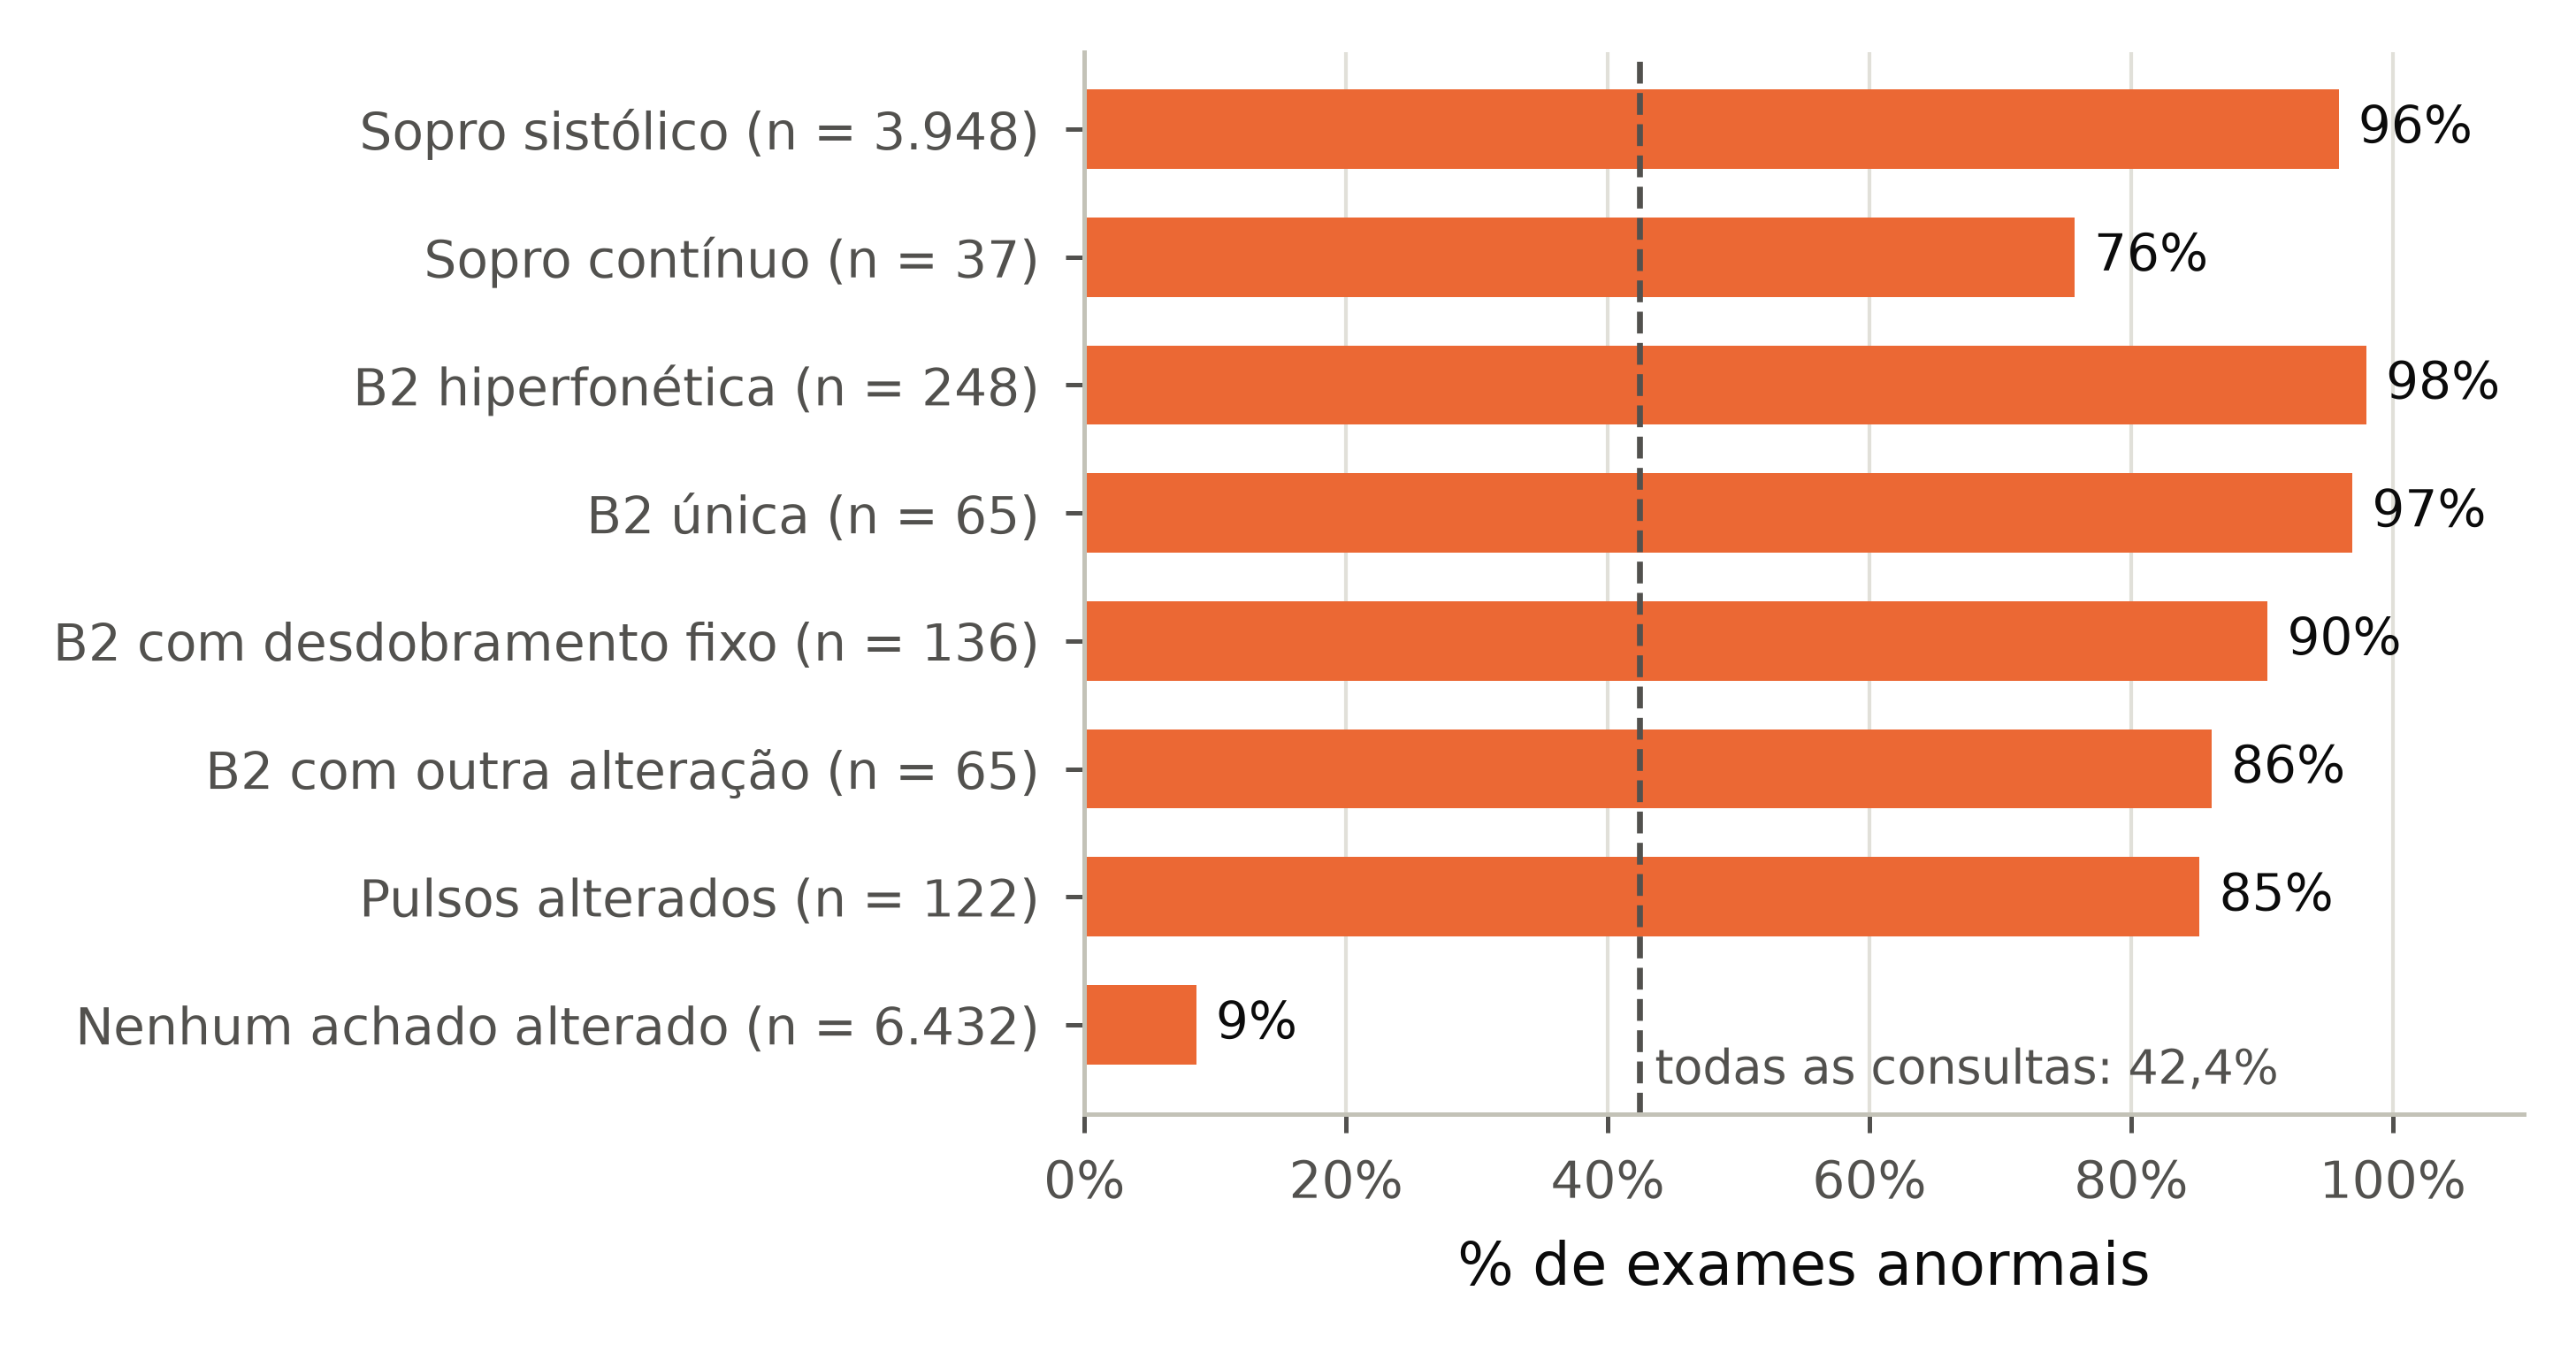
\includegraphics[width=\columnwidth]{fig1_vazamento_exame_fisico}
\caption{Proporção de laudos anormais em cada achado do exame físico, na base limpa. A linha tracejada marca a proporção do conjunto completo. Achados registrados no mesmo exame que produz o rótulo separam as classes quase perfeitamente, sinal de vazamento de informação.}
\label{fig:vazamento}
\end{figure}

Entre os atributos que podem ser usados, dois se destacam (Fig.~\ref{fig:alvo}). O primeiro é a idade: a proporção de laudos anormais cai de 61,2\% no primeiro ano de vida para 27,9\% entre 15 e 19 anos. O segundo, que separa as classes ainda melhor, é o motivo do encaminhamento. As consultas por cardiopatia já estabelecida chegam a 71,2\% de laudos anormais, contra 25,2\% nos pedidos de parecer cardiológico, o motivo mais frequente da base (4.795 consultas).

\begin{figure}[!t]
\centering
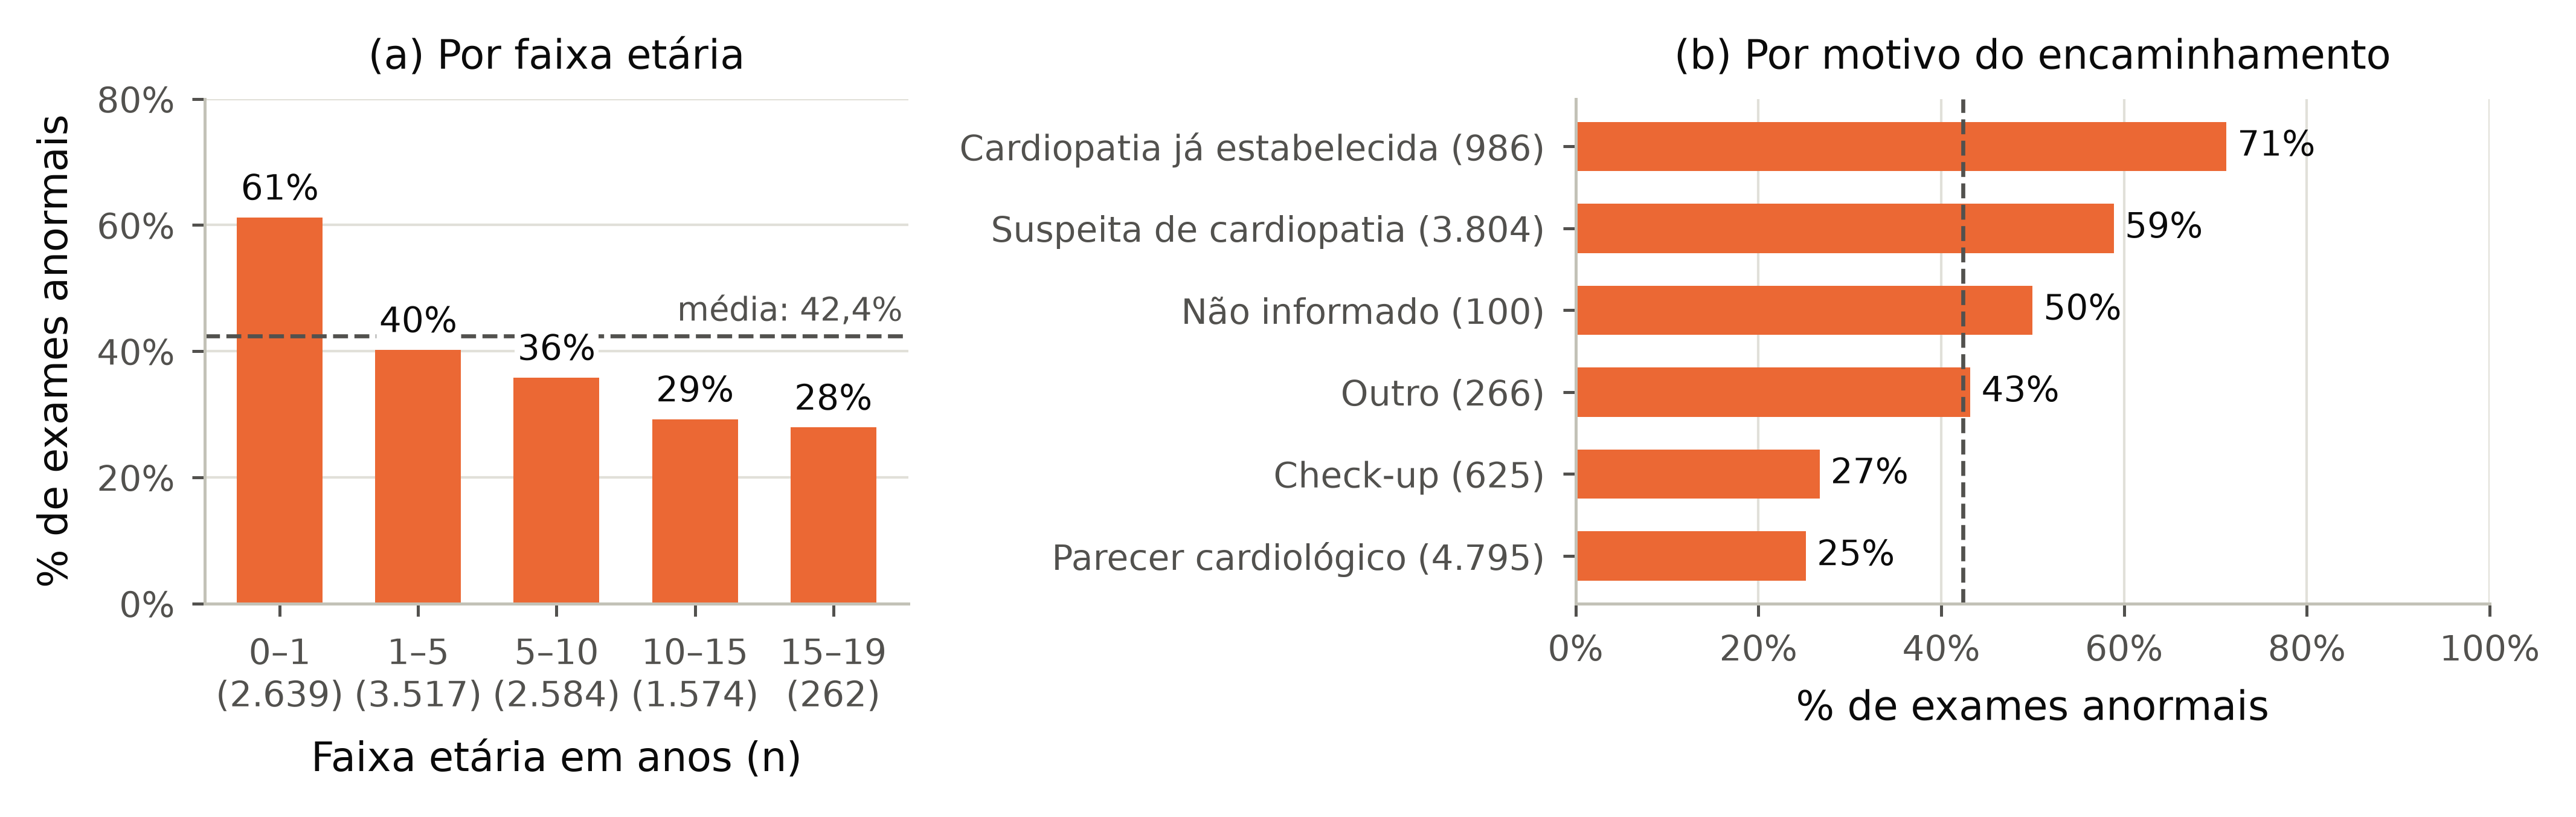
\includegraphics[width=\columnwidth]{fig2_alvo_idade_motivo}
\caption{Proporção de laudos anormais por faixa etária (a) e por motivo principal do encaminhamento (b), na base limpa, com o número de consultas entre parênteses. São as duas informações anteriores à consulta que mais pesam nos modelos.}
\label{fig:alvo}
\end{figure}

\section{Metodologia}
\subsection{Pré-processamento}
A limpeza feita na A1 removeu 2.297 consultas: 1.579 sem idade recuperável, 380 sem alvo e as demais por duplicidade, idade fora de 0 a 19 anos, idade incompatível com peso e altura ou excesso de valores ausentes. Nessa etapa, valores de peso e altura implausíveis para a idade e o sexo também foram tratados como ausentes, com base nas curvas de crescimento do CDC \cite{cdc}. Peso e altura ficam de fora dos modelos por serem redundantes com a idade (correlação de Spearman de 0,97 e 0,99), e o IMC, recalculado a partir deles, é mantido. A idade passa por uma transformação logarítmica antes de ser padronizada, o que reduz a assimetria de 0,76 para $-$0,25. Frequência cardíaca e pressão arterial são padronizadas dentro de cada faixa etária, para separar o seu efeito do efeito da idade, e os valores ausentes dessas variáveis e do IMC são imputados pela mediana da faixa. A pressão arterial, classificada segundo o \textit{Fourth Report} \cite{fourth}, entra como variável ordinal com dois indicadores de ausência. Sexo, sintomas e motivo do encaminhamento viram indicadores binários (uma consulta pode ter mais de um sintoma ou motivo), e as categorias com menos de 30 casos são agrupadas.

Tão importante quanto essas regras é o momento em que elas são ajustadas. Medianas, médias, desvios-padrão, modas e a lista de categorias frequentes são aprendidas dos dados, e calculá-las na base inteira antes de separar treino e validação levaria informação de um conjunto para o outro. Para evitar isso, o pré-processador foi implementado como transformador do scikit-learn \cite{sklearn} e incluído em um \textit{pipeline}, de modo que é reajustado em cada dobra usando apenas as linhas de ajuste daquela dobra.

\subsection{Protocolo de validação}
A base foi dividida em 8.460 consultas de treino e 2.116 de teste, com 42,4\% de laudos anormais em cada parte. O teste é uma das cinco partições de uma divisão estratificada, e não um corte aleatório isolado. Hiperparâmetros, escolha do modelo e limiar de decisão foram definidos por validação cruzada estratificada de cinco dobras dentro do treino. O teste só foi usado uma vez, depois de todas essas decisões, e nenhum resultado dele alterou qualquer escolha.

A etapa anterior previa agrupar a divisão por uma chave formada pela data de atendimento e pela data de nascimento, supondo que ela identificasse o paciente. A verificação feita aqui não confirma essa suposição. Dos 160 grupos com mais de uma consulta, 31 reúnem registros de sexos diferentes e 42 reúnem laudos diferentes, ou seja, são crianças distintas atendidas no mesmo dia. Como a base não tem identificador de paciente, cada consulta foi tratada como uma observação independente, e a possibilidade de consultas repetidas aparece entre as limitações do estudo.

Uma estimativa feita em um único conjunto de teste depende da partição sorteada. Por isso, o resultado principal foi confirmado por validação cruzada aninhada nas 10.576 consultas \cite{varma}, com cinco dobras externas para avaliação e três internas para a escolha de hiperparâmetros. Nesse protocolo, nenhuma observação participa ao mesmo tempo da escolha e da avaliação, e a estimativa não depende de um corte específico.

\subsection{Algoritmos e métricas}
O primeiro algoritmo, a classe majoritária, só fixa o piso: prevê sempre ``normal'' e não aprende nada. A regressão logística é o modelo simples exigido, linear e aditivo, com coeficientes que podem ser auditados um a um. Random Forest \cite{breiman} e Gradient Boosting por histogramas \cite{friedman} são os modelos complexos, capazes de representar efeitos não lineares e interações. O primeiro combina centenas de árvores ajustadas a amostras diferentes, o que reduz a variância; o segundo ajusta árvores pequenas em sequência, cada uma corrigindo o erro acumulado das anteriores, o que reduz o viés. Os hiperparâmetros foram escolhidos por busca em grade (57 combinações no total), sempre dentro do treino, pela área sob a curva ROC (AUC) média das dobras. Os valores escolhidos foram C = 0,1 na regressão logística, folhas com pelo menos 5 consultas no Random Forest e taxa de aprendizado de 0,05, com até 31 folhas por árvore, no Gradient Boosting.

A AUC foi a métrica de seleção porque não depende do limiar de decisão e mede diretamente a qualidade da ordenação, que é o uso pretendido. Entre as métricas que dependem do limiar, a sensibilidade para a classe anormal tem prioridade clínica, já que deixar de sinalizar uma criança com alteração cardíaca é mais grave do que um encaminhamento desnecessário. Para cada modelo, o limiar foi fixado no maior valor que alcança sensibilidade de 0,80 nas previsões \textit{out-of-fold} do treino e só depois aplicado ao teste. A importância dos atributos foi medida por permutação, e não pela redução de impureza das árvores, que favorece atributos com muitos valores distintos. A permutação também foi feita por grupo temático, porque atributos que descrevem a mesma informação se compensam quando são embaralhados um a um.

\section{Resultados e Discussão}
\begin{table}[!t]
\caption{Desempenho no cenário com 37 atributos. A coluna de validação cruzada traz a média e o desvio-padrão das cinco dobras do treino; as demais referem-se ao conjunto de teste (2.116 consultas), com intervalos de 95\% por reamostragem \textit{bootstrap}. Sensibilidade, especificidade e F1 usam o limiar fixado no treino.}
\label{tab:comparativa}
\centering
\footnotesize
\setlength{\tabcolsep}{3pt}
\resizebox{\columnwidth}{!}{%
\begin{tabular}{lcccccc}
\toprule
modelo & AUC val. cruz. & AUC teste & IC 95\% & sens. & espec. & F1 \\
\midrule
Classe majoritária & 0,500 $\pm$ 0,000 & 0,500 & --- & --- & --- & --- \\
Regressão logística & 0,764 $\pm$ 0,008 & 0,792 & 0,772 a 0,811 & 0,821 & 0,574 & 0,684 \\
Random Forest & 0,775 $\pm$ 0,013 & 0,803 & 0,784 a 0,821 & 0,810 & 0,614 & 0,694 \\
Gradient Boosting & 0,777 $\pm$ 0,015 & 0,802 & 0,784 a 0,821 & 0,810 & 0,624 & 0,698 \\
\bottomrule
\end{tabular}}
\end{table}

Os três modelos superam com folga o piso da classe majoritária, mas ficam próximos entre si (Tabela~\ref{tab:comparativa} e Fig.~\ref{fig:roc}). Na validação cruzada, que é o critério de seleção, o Gradient Boosting alcança 0,777 e a regressão logística, 0,764, uma vantagem de 0,012. No teste, a reamostragem \textit{bootstrap} pareada \cite{efron}, que avalia os dois modelos nas mesmas consultas sorteadas, mostra que essa vantagem é pequena, mas consistente: a diferença é positiva em 98,0\% das reamostragens. Entre os dois modelos complexos, a diferença não se distingue de zero (intervalo de $-$0,007 a 0,005).

A AUC do Gradient Boosting no teste (0,802) ficou acima da obtida na validação cruzada (0,777), o que sugere uma partição favorável, e não um ganho real. A validação cruzada aninhada, que usa as 10.576 consultas e não depende de um único corte, fica entre os dois valores, com 0,786 $\pm$ 0,013. É essa a estimativa que o trabalho adota como desempenho esperado.

\begin{figure}[!t]
\centering
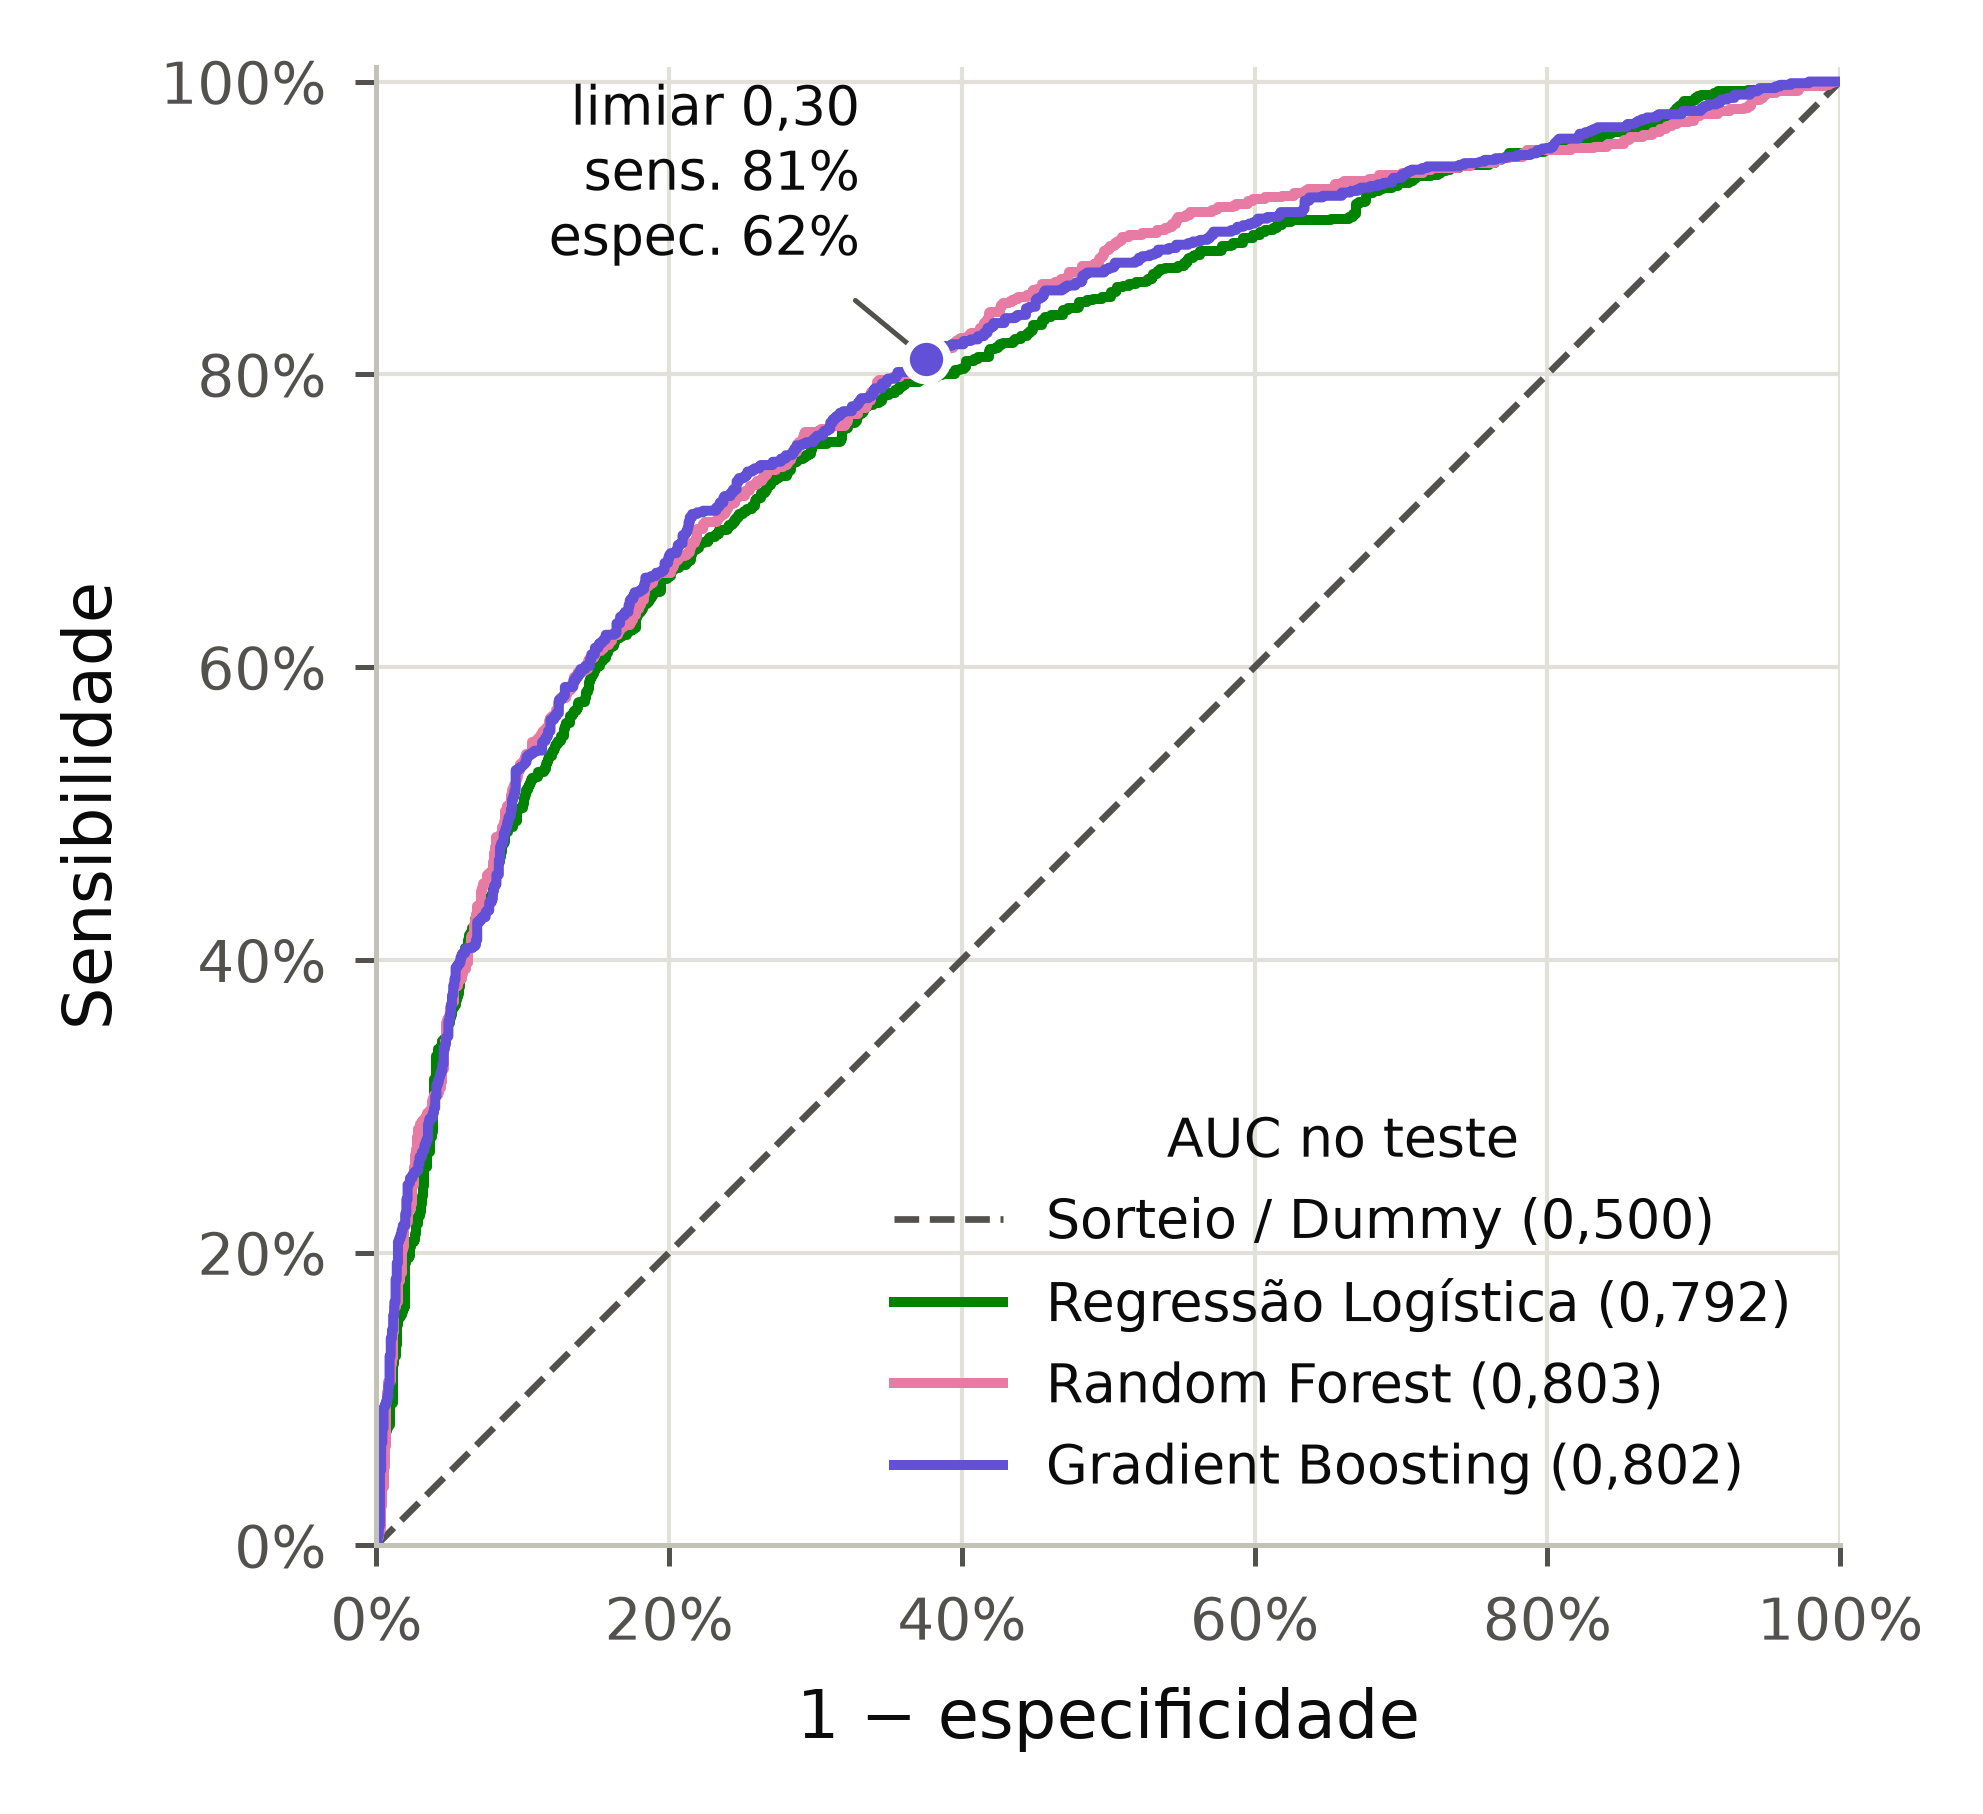
\includegraphics[width=0.85\columnwidth]{fig4_roc_teste}
\caption{Curvas ROC no conjunto de teste. A diagonal corresponde ao desempenho de um sorteio. O ponto destacado marca o limiar fixado no treino para o modelo escolhido. As três curvas praticamente se sobrepõem: a vantagem dos modelos complexos não se concentra em nenhuma faixa de limiar.}
\label{fig:roc}
\end{figure}

\subsection{O custo de excluir o exame físico}
A Fig.~\ref{fig:regua} responde à pergunta central do trabalho. Com os achados do exame físico, a AUC do Gradient Boosting na validação cruzada é de 0,950; sem eles, cai para 0,777. Essa queda de 0,174 não representa perda de capacidade preditiva, e sim o quanto do laudo já estava contido naqueles atributos. Um modelo com AUC de 0,95 pareceria excelente, mas seria inútil, porque depende justamente da informação que a triagem não tem. Retirando também o motivo do encaminhamento, a AUC cai para 0,674, o que mostra quanto se consegue apenas com o que é medido na própria consulta.

\begin{figure}[!t]
\centering
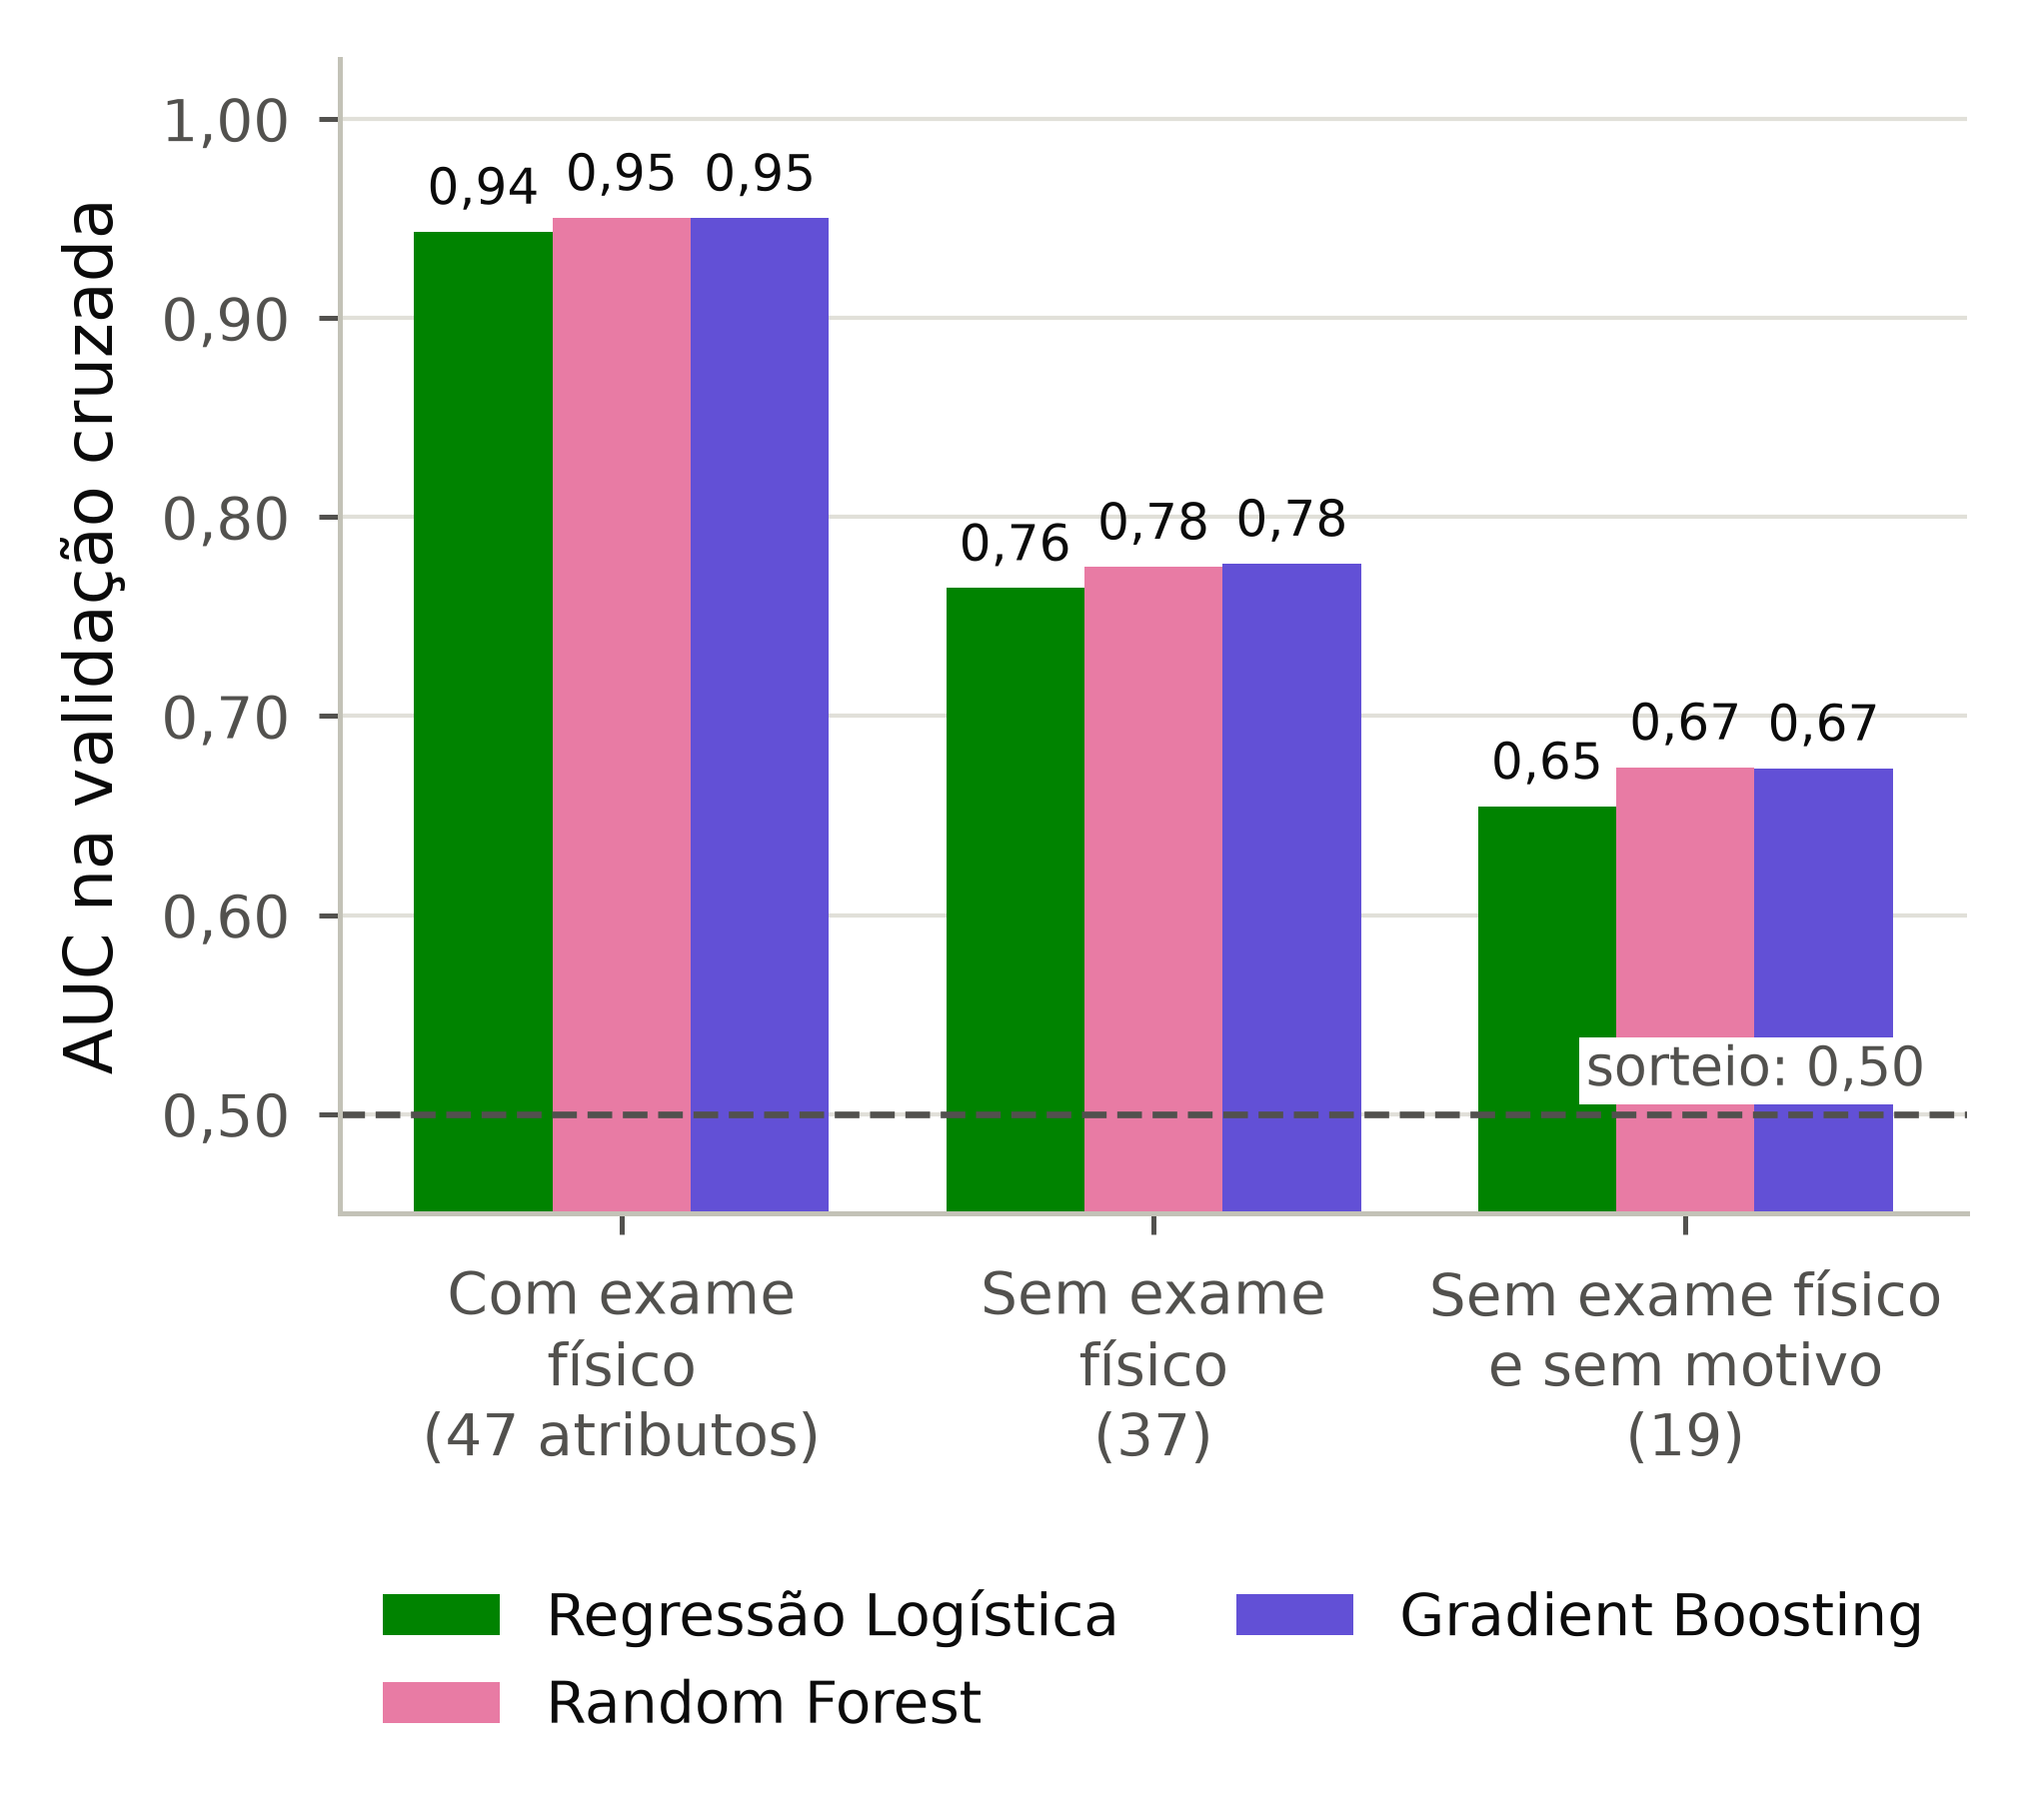
\includegraphics[width=0.85\columnwidth]{fig3_regua_vazamento}
\caption{Área sob a curva ROC na validação cruzada do treino, por conjunto de atributos. O primeiro grupo de barras inclui os achados do exame físico e serve apenas de régua para medir o vazamento; o segundo é o cenário adotado; o terceiro remove também o motivo do encaminhamento.}
\label{fig:regua}
\end{figure}

\subsection{Análise dos erros}
No limiar fixado no treino (0,30), o Gradient Boosting encontra 727 dos 897 laudos anormais do teste (81,0\%) e deixa passar 170 (Tabela~\ref{tab:confusao}). Entre os 1.219 laudos normais, prioriza 458 (37,6\%) e libera 761. Essa assimetria é intencional: exigir sensibilidade alta gera cerca de 2,7 falsos alarmes para cada laudo anormal perdido. Na prática, a fila priorizada reúne 1.185 consultas, 61,4\% delas anormais, e a fila liberada reúne 931, com 18,3\% de anormais, menos da metade da proporção da base.

\begin{table}[!t]
\caption{Matriz de confusão do modelo escolhido no conjunto de teste, no limiar fixado no treino. Os percentuais são por linha, isto é, sobre o total de cada classe real.}
\label{tab:confusao}
\centering
\footnotesize
\begin{tabular}{>{\raggedright\arraybackslash}p{2.3cm}cc}
\toprule
Gradient Boosting, limiar 0,30 & \shortstack{Liberado\\(previsto Normal)} & \shortstack{Priorizado\\(previsto Anormal)} \\
\midrule
Real: Normal & 761 (62,4\%) & 458 (37,6\%) \\
Real: Anormal & 170 (19,0\%) & 727 (81,0\%) \\
\bottomrule
\end{tabular}
\end{table}

Aumentar a sensibilidade custa cada vez mais. Nas previsões \textit{out-of-fold} do treino, passar de 0,75 para 0,80 eleva a fração de crianças priorizadas de 52,8\% para 59,7\%, e chegar a 0,90 exigiria priorizar 76,9\%, ponto em que a triagem praticamente deixaria de triar. Por isso, o ponto de operação é uma decisão clínica, e não estatística. O modelo fornece a curva inteira, e o valor de 0,80 adotado aqui é uma convenção de trabalho.

Os erros não se distribuem de maneira uniforme. Por faixa etária (Tabela~\ref{tab:faixa}), a sensibilidade cai de 0,96 no primeiro ano de vida para 0,46 entre 15 e 19 anos, enquanto a especificidade sobe de 0,31 para 0,95. O modelo acompanha a prevalência de cada faixa: prioriza quase todos os bebês, dos quais 60,0\% têm laudo anormal, e quase nenhum adolescente. Os valores da última faixa, porém, vêm de apenas 52 consultas.

\begin{table}[!t]
\caption{Desempenho do modelo escolhido por faixa etária, no conjunto de teste e no limiar fixado no treino. A última coluna traz o número de laudos anormais não detectados em cada faixa.}
\label{tab:faixa}
\centering
\footnotesize
\begin{tabular}{lccccc}
\toprule
faixa (anos) & n & \% An. & sens. & espec. & An. perdidos \\
\midrule
0--1 & 543 & 60,0 & 0,963 & 0,313 & 12 \\
1--5 & 696 & 41,8 & 0,804 & 0,635 & 57 \\
5--10 & 515 & 35,3 & 0,670 & 0,667 & 60 \\
10--15 & 310 & 27,4 & 0,600 & 0,787 & 34 \\
15--19 & 52 & 25,0 & 0,462 & 0,949 & 7 \\
\bottomrule
\end{tabular}
\end{table}

A diferença é ainda maior entre os motivos do encaminhamento (Fig.~\ref{fig:motivo}). Nas 178 consultas por cardiopatia já estabelecida, a sensibilidade é de 0,98; nas 970 de parecer cardiológico, que têm apenas 24,4\% de laudos anormais, cai para 0,48. Essas consultas de parecer concentram 124 dos 170 laudos anormais não detectados (73\%).

Esse é o principal achado do trabalho. Na prática, o modelo funciona como um resumo quantitativo do encaminhamento e da idade: ordena bem as crianças que já chegam com suspeita e falha justamente nos pedidos de rotina, em que a alteração só aparece no exame. Uma triagem automatizada desse tipo adiantaria crianças que a simples leitura do encaminhamento já priorizaria e acrescentaria pouco onde mais seria necessária.

\begin{figure}[!t]
\centering
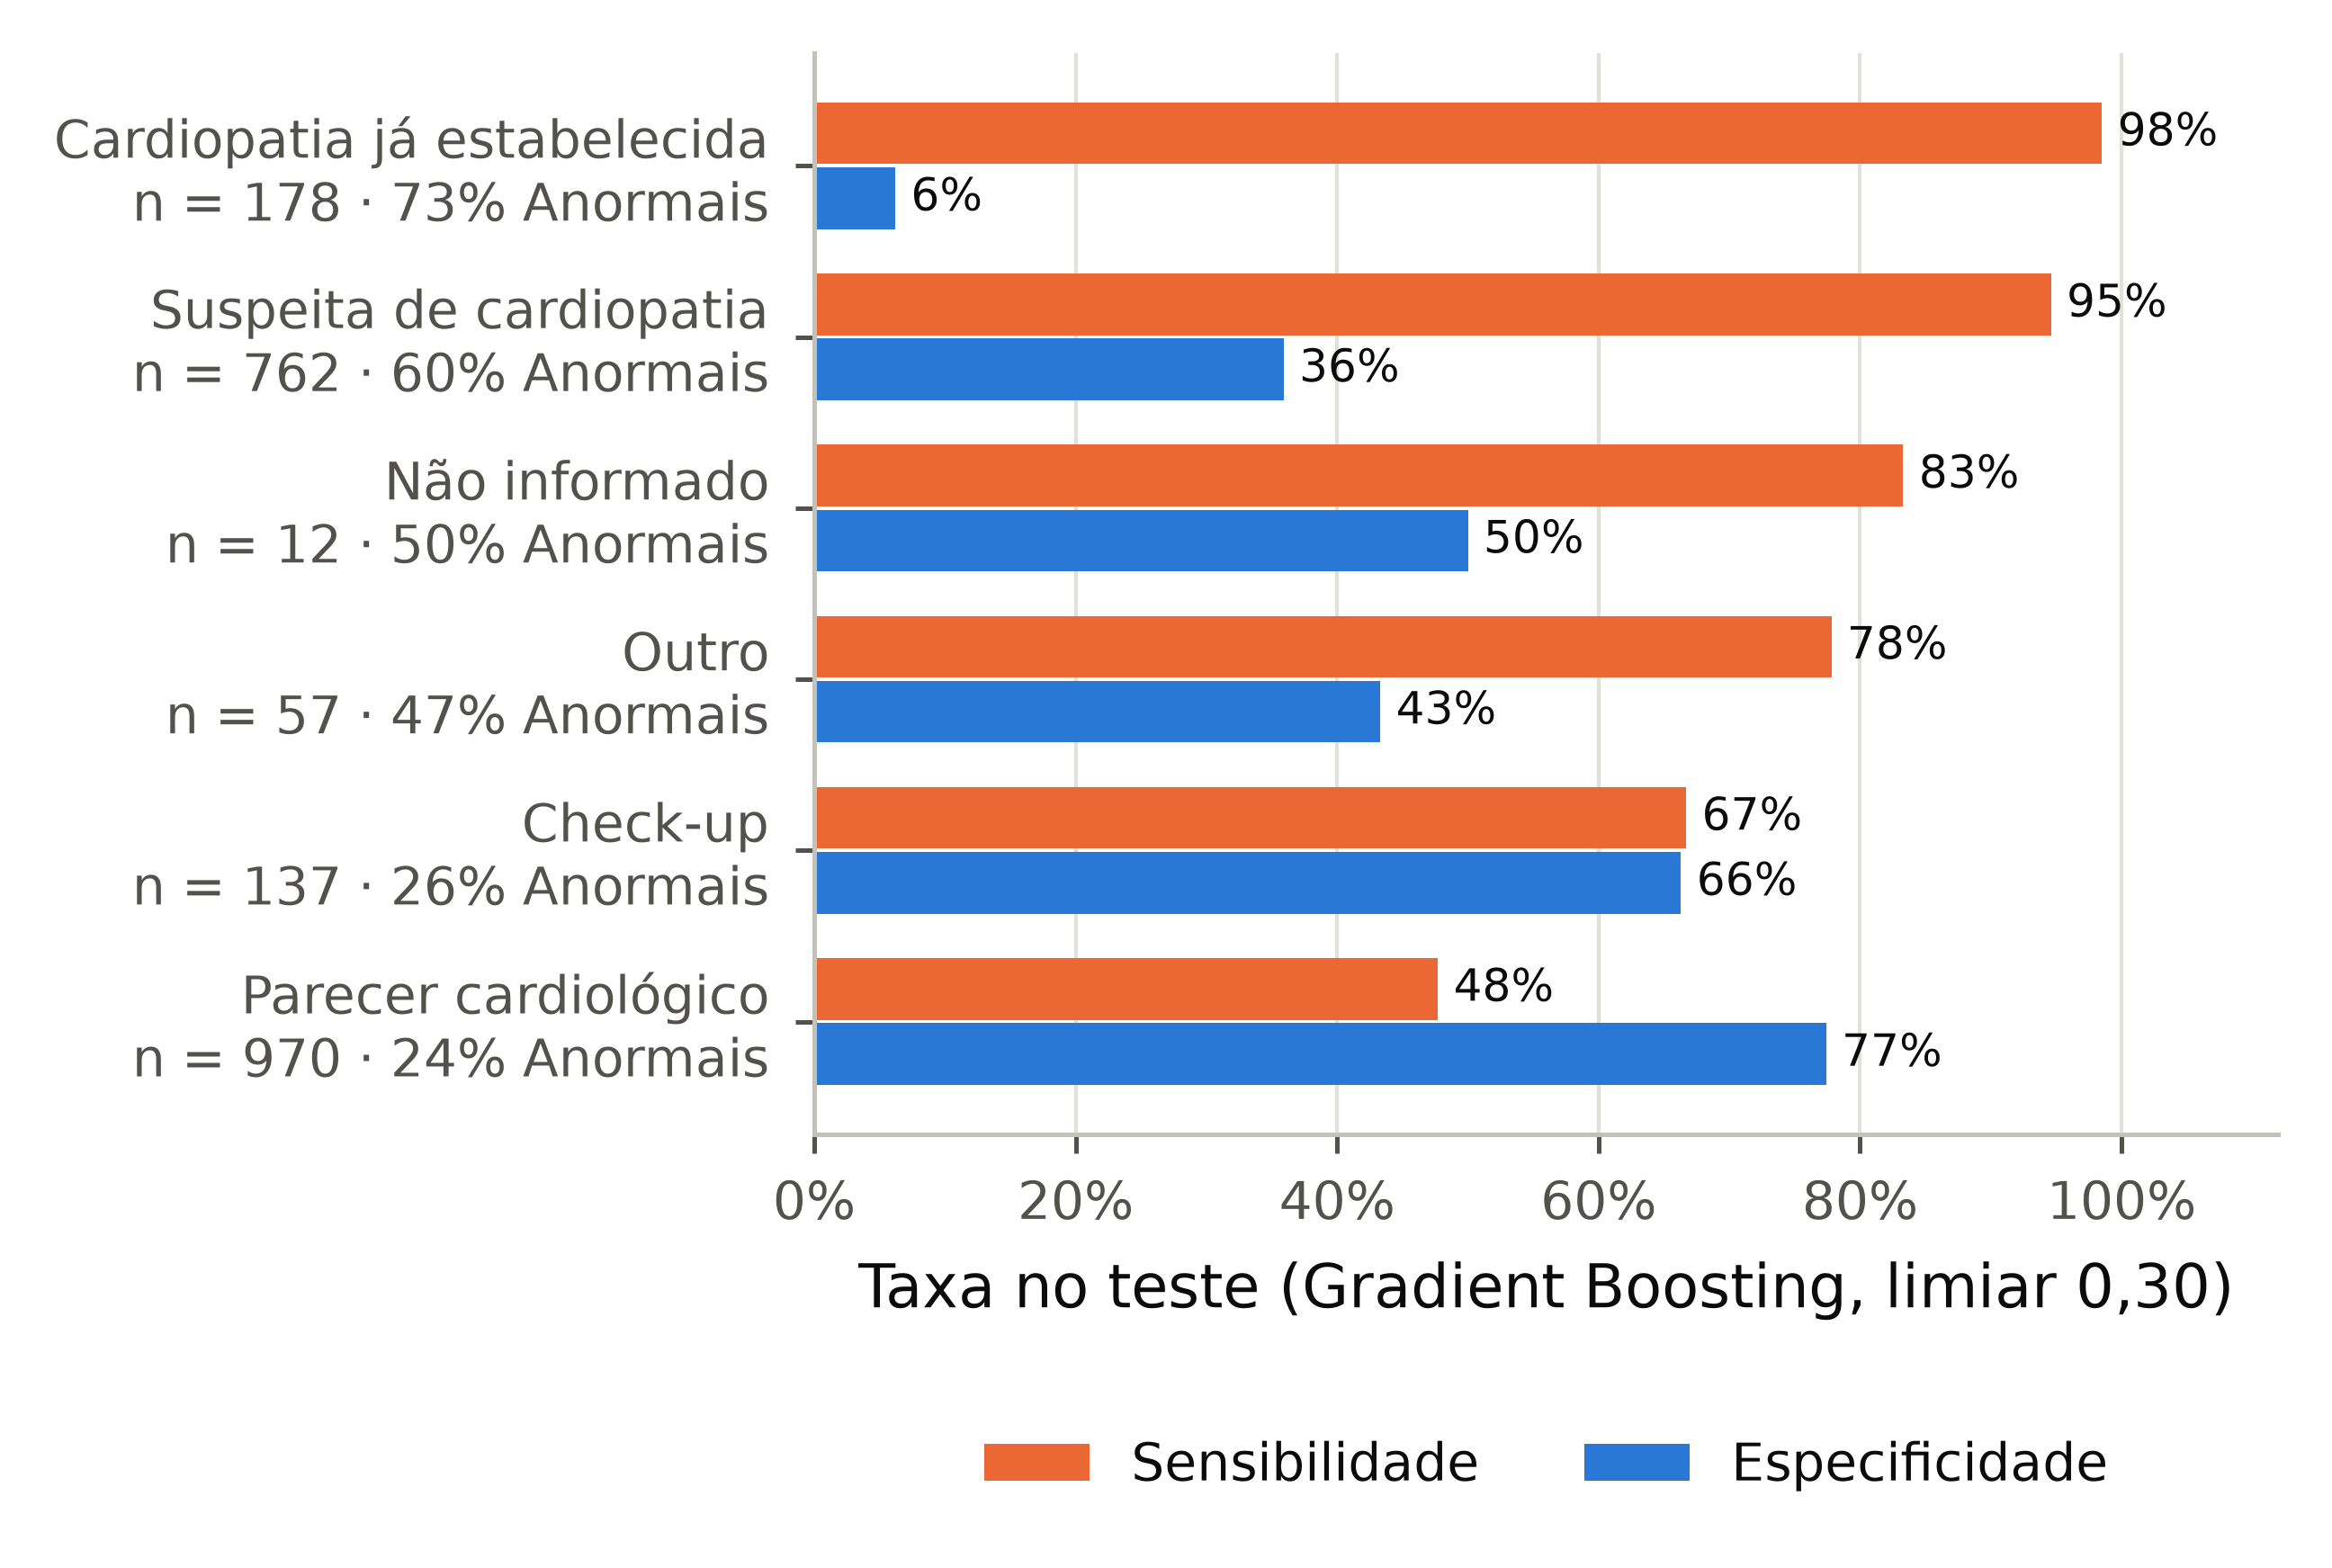
\includegraphics[width=\columnwidth]{fig6_erros_por_motivo}
\caption{Sensibilidade e especificidade do modelo escolhido no conjunto de teste, por motivo principal do encaminhamento, no limiar fixado no treino. Os rótulos trazem o número de consultas e a proporção de laudos anormais de cada grupo.}
\label{fig:motivo}
\end{figure}

\subsection{Importância dos atributos}
A importância por grupo (Fig.~\ref{fig:importancia}) é muito concentrada. Embaralhar as 18 colunas do motivo do encaminhamento derruba a AUC em 0,204, enquanto nenhum outro grupo passa de 0,028, valor alcançado pela idade. Nos três modelos, o motivo do encaminhamento fica muito à frente dos demais grupos, o que indica que esse resultado reflete os dados, e não o algoritmo. Entre os atributos individuais, o mais importante é o encaminhamento por sopro (0,083), seguido pela frequência cardíaca e pela idade.

Os coeficientes da regressão logística mostram a direção dos efeitos. Os encaminhamentos que já trazem suspeita aumentam a chance de laudo anormal: sopro (razão de chances de 3,21), cardiopatia já estabelecida (1,94) e cardiopatia congênita (1,76). Os pedidos de rotina, como parecer cardiológico (0,53) e check-up (0,53), a reduzem. Pressão arterial, IMC e sexo têm efeito desprezível, como a análise bivariada da etapa anterior já indicava.

\begin{figure}[!t]
\centering
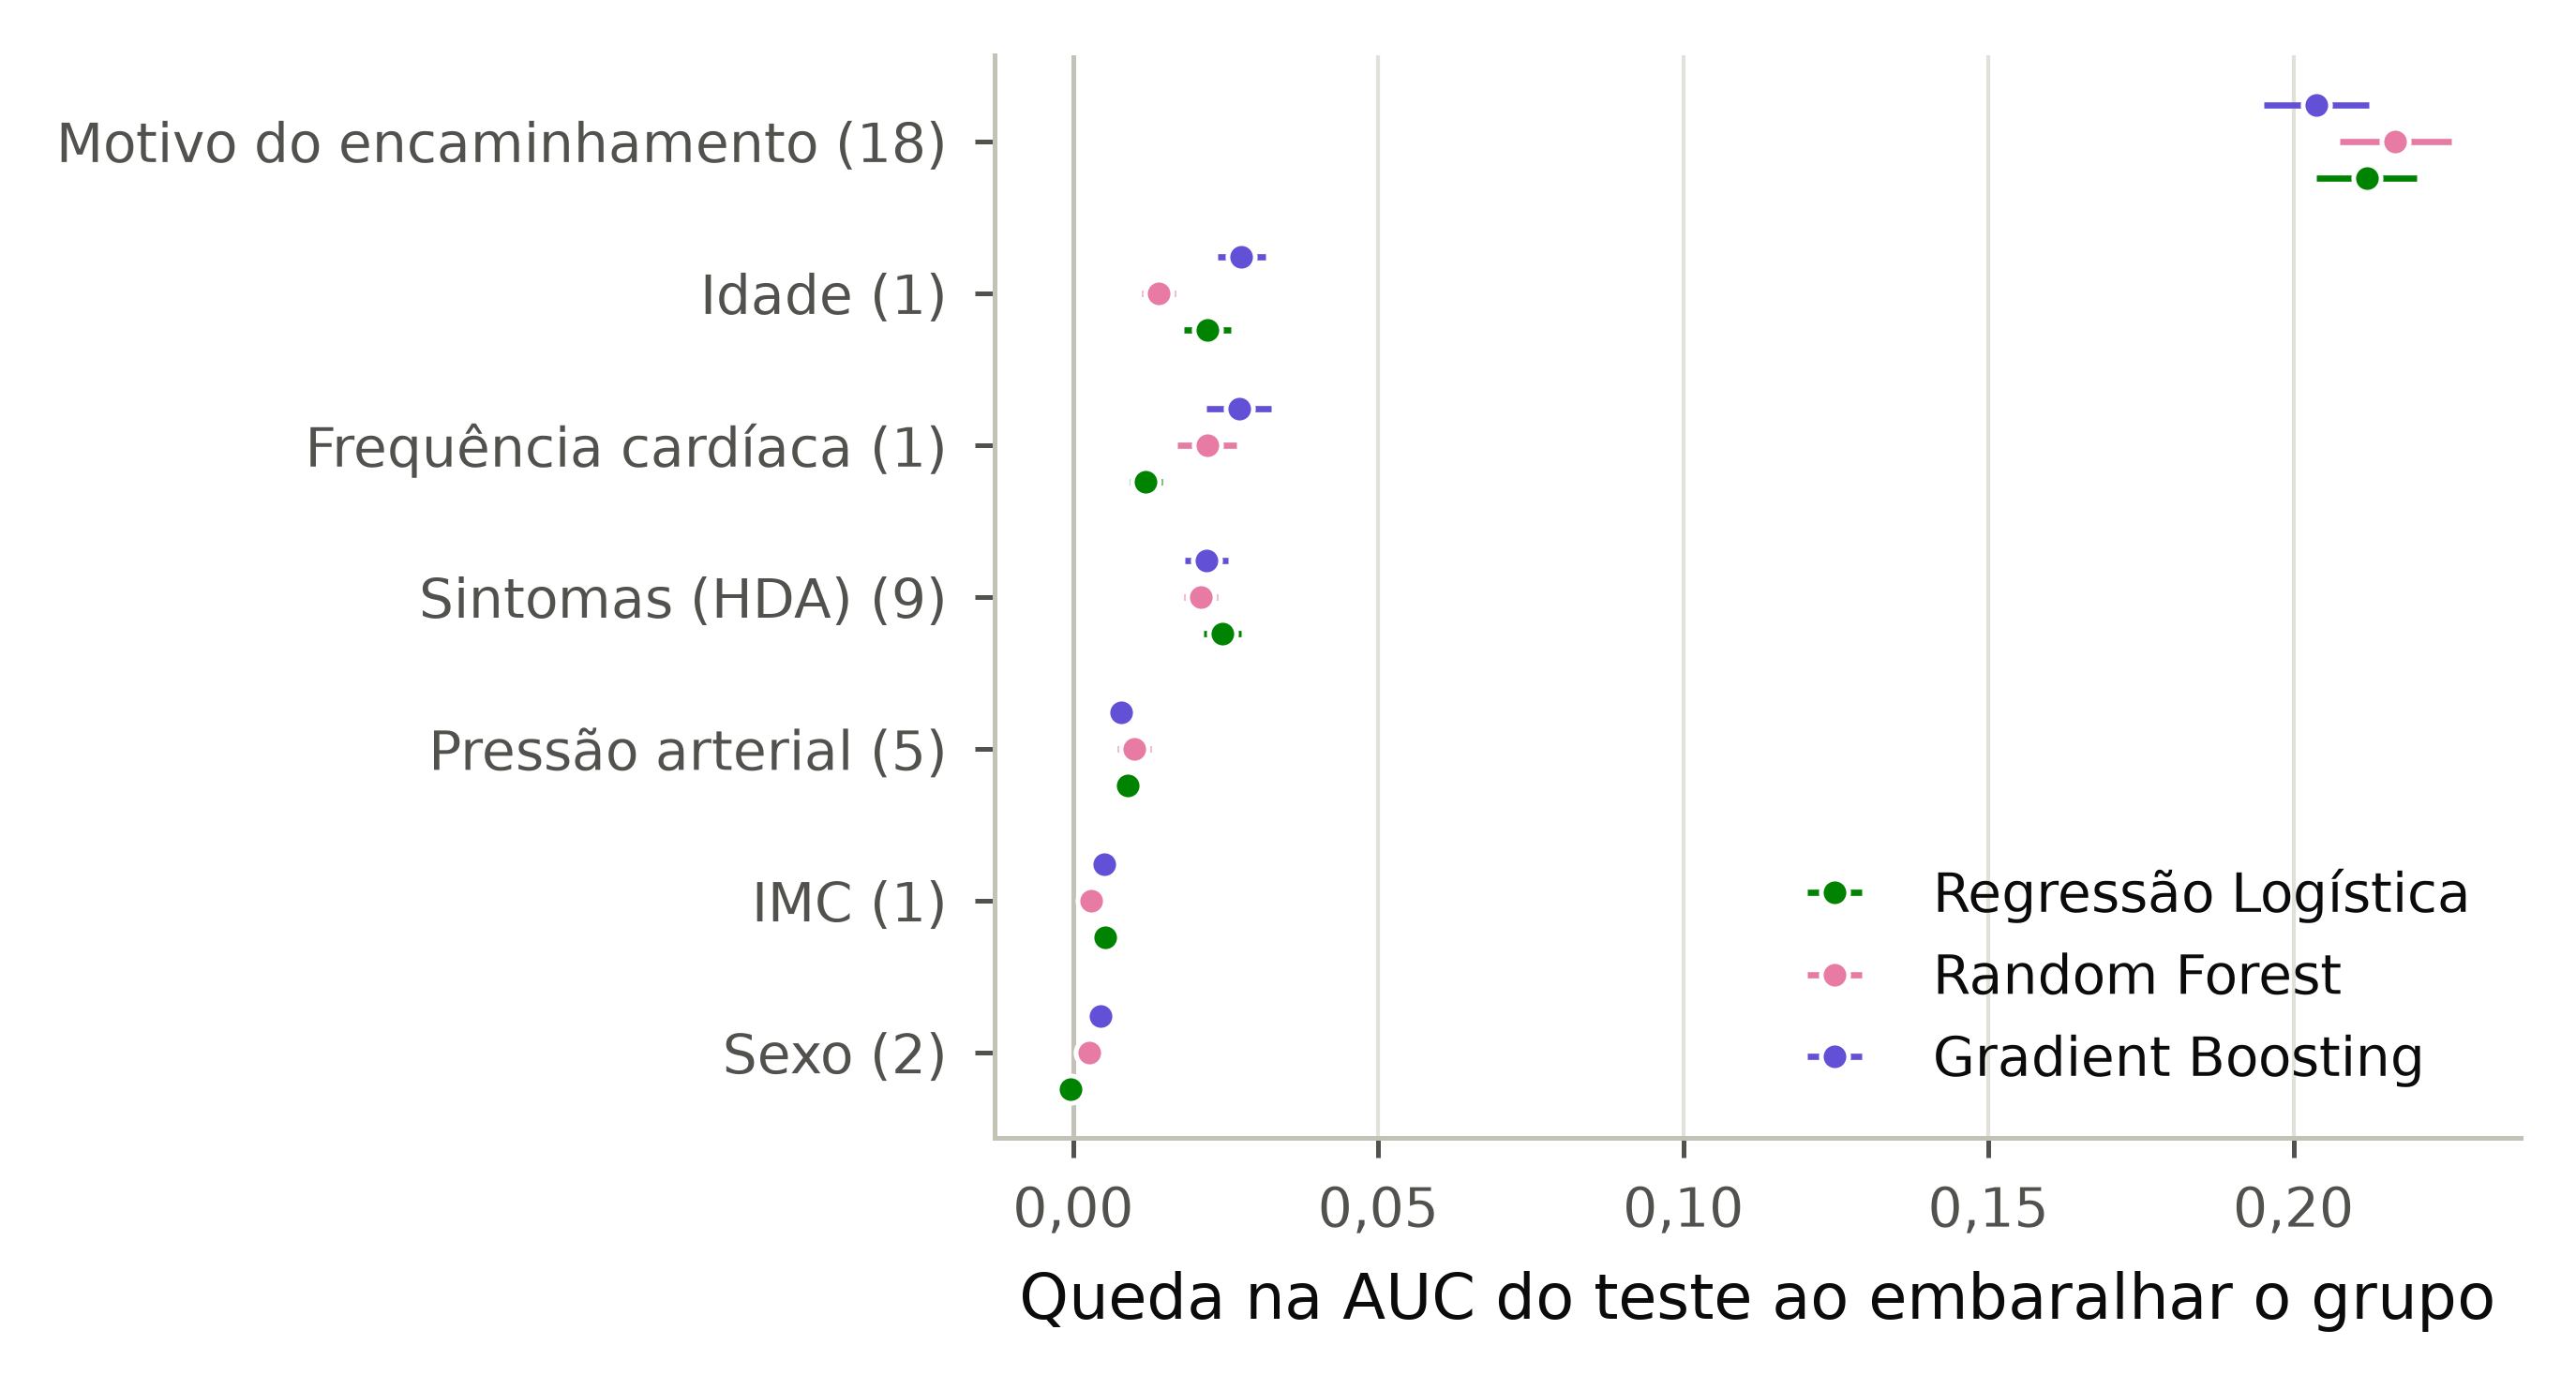
\includegraphics[width=\columnwidth]{fig5_importancia_grupos}
\caption{Queda na área sob a curva ROC do teste ao embaralhar, em conjunto, as colunas de cada grupo temático (média de 30 repetições, barras de desvio-padrão). Entre parênteses, o número de colunas do grupo.}
\label{fig:importancia}
\end{figure}

\subsection{Robustez e limitações}
A proporção de laudos anormais cai ao longo da série histórica, de 55,8\% em 2003 para 28,6\% em 2010, o que sugere mudança no perfil dos atendimentos. Como a validação cruzada sorteia as dobras e mistura os anos, o experimento foi repetido com uma divisão temporal, treinando até 2007 e validando de 2008 em diante (Tabela~\ref{tab:temporal}). Nessa divisão, a AUC do Gradient Boosting é de 0,764, cerca de 0,02 abaixo da validação cruzada aninhada (0,786), e a capacidade de ordenar se mantém. Já a regressão logística (0,771) supera o Gradient Boosting, o que reforça que a vantagem dos modelos complexos é frágil. A prevalência menor no período final (37,7\%, contra 42,4\% na base) não altera a AUC, mas faz um limiar fixado no passado perder precisão.

\begin{table}[!t]
\caption{AUC da regressão logística e do Gradient Boosting sob três protocolos: o teste sorteado, a validação cruzada aninhada na base inteira e uma divisão temporal. Como a AUC não depende da prevalência, a queda na divisão temporal provavelmente reflete a mudança no perfil dos atendimentos e o treino menor (6.072 consultas).}
\label{tab:temporal}
\centering
\footnotesize
\setlength{\tabcolsep}{3pt}
\begin{tabular}{>{\raggedright\arraybackslash}p{3.0cm}cccc}
\toprule
protocolo & valid. (n) & \% An. & logística & boosting \\
\midrule
teste sorteado (80/20) & 2.116 & 42,4 & 0,792 & 0,802 \\
validação cruzada aninhada 5$\times$3 & 10.576 & 42,4 & 0,771 & 0,786 \\
divisão temporal (treino até 2007) & 4.497 & 37,7 & 0,771 & 0,764 \\
\bottomrule
\end{tabular}
\end{table}

Três limitações restringem o alcance desses resultados. Primeiro, a base não tem identificador de paciente, então consultas repetidas da mesma criança, se existirem, podem ficar em lados diferentes da divisão. Segundo, o perfil dos atendimentos muda ao longo dos anos, e o desempenho medido vale para a distribuição observada. Por fim, o rótulo é o laudo de um cardiologista, e não um desfecho confirmado por exame complementar, de modo que o modelo aprende a reproduzir um julgamento clínico, com a variabilidade que lhe é própria.

\section{Conclusão}
Sem os achados do exame físico, a AUC caiu de 0,95 para 0,78, e a validação cruzada aninhada na base completa estima 0,786 para o melhor modelo. Juntos, esses números resumem o trabalho: o desempenho aparentemente excelente do primeiro cenário vinha de atributos anotados no mesmo ato clínico que gera o rótulo, e o desempenho realista, sem eles, é moderado.

A vantagem do melhor modelo complexo sobre a regressão logística foi de 0,012 de AUC, enquanto a exclusão do exame físico respondeu por uma queda de 0,174, cerca de 14 vezes maior. O limite do problema está na informação disponível antes da consulta, e não na escolha do algoritmo. Em uso clínico, a regressão logística seria uma escolha defensável pela interpretabilidade, já que a diferença para o Gradient Boosting é pequena e se inverte na divisão temporal.

Como ferramenta de triagem, a utilidade é parcial: o modelo ordena bem as crianças que chegam com suspeita registrada no encaminhamento, mas é fraco nos pedidos de rotina, onde estão 73\% dos laudos anormais que ele deixa passar. Três caminhos parecem promissores para dar continuidade ao trabalho: incorporar informações anteriores à consulta que a base não contém, como histórico familiar e dados do pré-natal; aproveitar o texto livre do encaminhamento, hoje reduzido a categorias; e validar o modelo em outro serviço, para separar o que é padrão clínico do que é característica da UCMF.

\section{Uso de Inteligência Artificial Generativa}
O assistente Claude (Anthropic) foi usado em quatro frentes, sempre a partir do protocolo definido pelo grupo: organização do repositório e da documentação; escrita do código de modelagem e das figuras; verificação da suposição de agrupamento por paciente descrita na Seção~III-B, que levou à correção adotada; e redação e revisão deste relatório, cuja primeira versão foi montada por um programa que lê as tabelas geradas pelo código. Os números apresentados não foram produzidos pelo assistente: todos vêm das tabelas exportadas pela execução do código, disponíveis no repositório. As decisões metodológicas, como quais atributos excluir, qual protocolo de validação adotar, quais algoritmos comparar e qual ponto de operação usar, foram tomadas pelo grupo e estão registradas no repositório.

% As referências estão na ordem da primeira citação, como exige o padrão IEEE.
\begin{thebibliography}{00}
\bibitem{dados} Unidade de Cardiologia e Medicina Fetal (UCMF), Real Hospital Português (RHP), ``UCMF\_raw: consultas de cardiologia pediátrica'', conjunto de dados anonimizado, Recife-PE. Fornecido pelo professor da disciplina Mineração de Dados, Instituto de Informática, Universidade Federal de Goiás, 2026.
\bibitem{kaufman} S. Kaufman, S. Rosset e C. Perlich, ``Leakage in data mining: formulation, detection, and avoidance'', ACM Transactions on Knowledge Discovery from Data, vol. 6, no. 4, pp. 1--21, 2012.
\bibitem{sklearn} F. Pedregosa et al., ``Scikit-learn: Machine learning in Python'', Journal of Machine Learning Research, vol. 12, pp. 2825--2830, 2011.
\bibitem{pandas} The pandas development team, ``pandas-dev/pandas: Pandas'', Zenodo, 2024. [Online]. Disponível em: \url{https://doi.org/10.5281/zenodo.3509134}
\bibitem{matplotlib} J. D. Hunter, ``Matplotlib: A 2D graphics environment'', Computing in Science \& Engineering, vol. 9, no. 3, pp. 90--95, 2007.
\bibitem{cdc} R. J. Kuczmarski et al., ``2000 CDC growth charts for the United States: methods and development'', Vital and Health Statistics, series 11, no. 246, National Center for Health Statistics, 2002.
\bibitem{fourth} National High Blood Pressure Education Program Working Group on High Blood Pressure in Children and Adolescents, ``The fourth report on the diagnosis, evaluation, and treatment of high blood pressure in children and adolescents'', Pediatrics, vol. 114, no. 2, pp. 555--576, 2004.
\bibitem{varma} S. Varma e R. Simon, ``Bias in error estimation when using cross-validation for model selection'', BMC Bioinformatics, vol. 7, no. 91, 2006.
\bibitem{breiman} L. Breiman, ``Random forests'', Machine Learning, vol. 45, no. 1, pp. 5--32, 2001.
\bibitem{friedman} J. H. Friedman, ``Greedy function approximation: a gradient boosting machine'', The Annals of Statistics, vol. 29, no. 5, pp. 1189--1232, 2001.
\bibitem{efron} B. Efron e R. J. Tibshirani, \textit{An Introduction to the Bootstrap}. New York: Chapman \& Hall, 1993.
\end{thebibliography}
\end{document}
